% Fig. 8 -- Four-model comparison on the 120 directly scoreable scenarios (single column, 3.5 in).
% Positive class = fabricated; bars = point estimates, whiskers = 95% Wilson intervals (none for F1).
% Numbers: paper/results.md (generated by paper/scripts/compute_results.py).
% Compile with pdfLaTeX (Overleaf default). Output: fig08_comparison.pdf
\documentclass[border=3pt]{standalone}
\usepackage[T1]{fontenc}
\usepackage{newtxtext,newtxmath}
\usepackage{tikz}
\usepackage{pgfplots}
\pgfplotsset{compat=1.17}

\definecolor{acc}{RGB}{31,78,121}

\pgfplotsset{
  barA/.style={ybar,fill=black!8, draw=black,line width=0.4pt,
    error bars/.cd,y dir=both,y explicit,error bar style={line width=0.4pt}},
  barB/.style={ybar,fill=black!30,draw=black,line width=0.4pt,
    error bars/.cd,y dir=both,y explicit,error bar style={line width=0.4pt}},
  barC/.style={ybar,fill=black!55,draw=black,line width=0.4pt,
    error bars/.cd,y dir=both,y explicit,error bar style={line width=0.4pt}},
  barD/.style={ybar,fill=acc,     draw=black,line width=0.4pt,
    error bars/.cd,y dir=both,y explicit,error bar style={line width=0.4pt}},
}

\begin{document}
\footnotesize
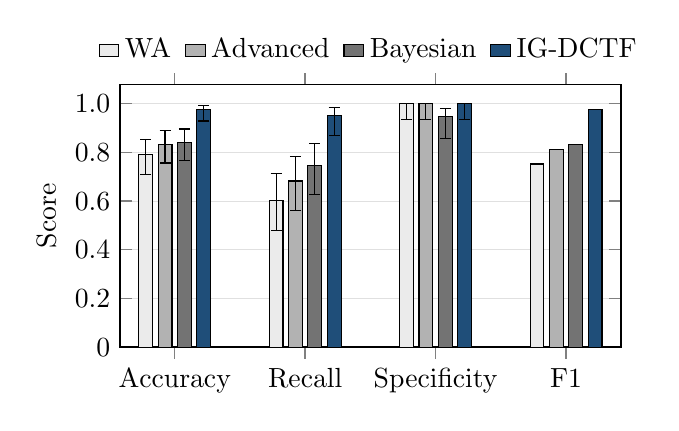
\begin{tikzpicture}
\begin{axis}[
    width=226pt, height=140pt,
    ybar, bar width=5pt,
    symbolic x coords={Accuracy,Recall,Specificity,F1},
    xtick=data,
    enlarge x limits=0.14,
    ymin=0, ymax=1.08,
    ytick={0,0.2,0.4,0.6,0.8,1.0},
    yticklabels={0,0.2,0.4,0.6,0.8,1.0},
    ylabel={Score},
    ymajorgrids, grid style={black!12,line width=0.3pt},
    axis line style={line width=0.5pt}, tick style={line width=0.5pt},
    legend style={at={(0.5,1.04)},anchor=south,legend columns=4,draw=none,
                  /tikz/every even column/.append style={column sep=3pt}},
    legend image code/.code={\draw[#1] (0cm,-0.08cm) rectangle (0.25cm,0.08cm);},
]
  % WA baseline
  \addplot[barA] coordinates {(Accuracy,0.7917) += (0,0.0630) -= (0,0.0812)
                              (Recall,0.6032)   += (0,0.1115) -= (0,0.1234)
                              (Specificity,1.0) += (0,0)      -= (0,0.0631)
                              (F1,0.7525)       += (0,0)      -= (0,0)};
  % Advanced (CVE-only)
  \addplot[barB] coordinates {(Accuracy,0.8333) += (0,0.0561) -= (0,0.0768)
                              (Recall,0.6825)   += (0,0.1016) -= (0,0.1225)
                              (Specificity,1.0) += (0,0)      -= (0,0.0631)
                              (F1,0.8113)       += (0,0)      -= (0,0)};
  % Bayesian
  \addplot[barC] coordinates {(Accuracy,0.8417) += (0,0.0545) -= (0,0.0758)
                              (Recall,0.7460)   += (0,0.0912) -= (0,0.1194)
                              (Specificity,0.9474) += (0,0.0345) -= (0,0.0911)
                              (F1,0.8319)       += (0,0)      -= (0,0)};
  % IG-DCTF
  \addplot[barD] coordinates {(Accuracy,0.9750) += (0,0.0165) -= (0,0.0459)
                              (Recall,0.9524)   += (0,0.0313) -= (0,0.0833)
                              (Specificity,1.0) += (0,0)      -= (0,0.0631)
                              (F1,0.9756)       += (0,0)      -= (0,0)};
  \legend{WA, Advanced, Bayesian, IG-DCTF}
\end{axis}
\end{tikzpicture}
\end{document}
